\documentclass{thesisreport}

\setcounter{tocdepth}{3}
\setcounter{secnumdepth}{3}

\usepackage{caption}
\usepackage{subcaption}
\usepackage{comment}
\usepackage{amsmath}
\usepackage{bm}
\usepackage{multicol}
\usepackage{xcolor}
\usepackage{tabularx}
\usepackage{optidef}
\usepackage{mathtools}

\setlength{\columnseprule}{1pt}
\def\columnseprulecolor{\color{black}}
\DeclareUnicodeCharacter{2212}{-}

\setlength\parindent{0pt}

\begin{document}

 \thispagestyle{empty}

\def\lskip{\vspace{0.5cm}}


\begin{tabular}{p{7cm}p{8cm}}
ÉCOLE CENTRALE DE NANTES
&
% EMARO students only
% \raggedleft FIRST YEAR INSTITUTION	
\end{tabular}

\vspace{2cm}

% CORO-IMARO students
\begin{center} \large\sc MASTER CORO-IMARO\\ \normalsize{``CONTROL and ROBOTICS''} \end{center}

% EMARO students
%\begin{center} \large\sc MASTER ERASMUS MUNDUS \\ \normalsize{EMARO+ ``European Master in Advanced Robotics''} \end{center}


\begin{center}
	2020 / 2021\\
	\lskip
	Master Thesis Report %Master Thesis Report % or bibliography report
	\lskip
	
	Presented by \lskip 
	
	Elie Hatem \lskip
	
	On \today \lskip\lskip
	
	{\Large \textbf{Making Flips With Quadrotors In Constrained Environments}}
	
	\vfill

Jury \lskip
		
	\end{center}
	


\begin{tabular}{p{3cm}p{7cm}p{5cm} }
 % President: & Name & Position (Institution) \\ & & \\     % for final defense only (not bibliography)
 Evaluators: & Dr. Olivier Kermorgant & Associate Professor (ECN) \\
	      & Dr. Damien SIX & Robotics Engineer (CNRS) \\ 
	      %& Name & Position (Institution) \\ & & \\  & & \\ 
  Supervisor(s):  & Dr. Sébastien Briot & Researcher (CNRS) \\
		  & Dr. Isabelle Fantoni & Research Director (CNRS) \\
% EMARO students only
%(EMARO)  & Co-supervisor from M1 & Position, M1 institution 
\end{tabular}

\lskip

\begin{flushleft}
 Laboratory: Laboratoire des Sciences du Numérique de Nantes LS2N
\end{flushleft}

\newpage
\thispagestyle{empty}
\null
\newpage
\addtocounter{page}{-1}
\pagestyle{fancy}
  
 
  \section*{Abstract}
   
Within the rapidly growing aerial robotics market, one of the most substantial challenges in the quadrotor community is performing aggressive maneuvers, especially multi-flip maneuvers.  A proper physical definition of the issue is not addressed by the current approaches in the field and several key aspects of this maneuver are still overlooked.
It can be shown, in particular, that making a flip with a quadrotor means crossing the parallel singularity of the dynamic model. The aim of the master thesis is to explore the possibility of defining aggressive trajectories for quadrotors on the basis of their dynamic model degeneracy analysis and to adapt various strategies to control the robot in a closed loop. In addition, the possibility of performing the aggressive maneuvers in constrained environments will also be investigated.
Therefore, the analysis will be extended from the previous studies to create general feasible trajectories that will allow quadrotors to perform aggressive multi-flip maneuvers while passing through a constrained environment and while guaranteeing a satisfactory degree of robustness to the uncertainties of the dynamic model.\\

\textbf{Keywords: quadrotors, parallel robots, aggressive maneuvers, multi-flips, constrained environmen. }
 
 
 \newpage
 
 \section*{Acknowledgements}
 
 I would like to express my special thanks and gratitude to my supervisors Dr. Sébastien Briot and Dr. Isabelle Fantoni who gave me the  opportunity to work on this wonderful project which encapsulates control theory, dynamics and quadrotors, which are all subjects that are very interesting for me. 
This project has allowed me to perform research on all of these topics and I am now more knowledgeable thanks to my supervisors. Moreover, I would like to thank them for believing in my capabilities and giving me the confidence and the support when I needed it. \\\\
I would like to thank my patient and understanding girlfriend Glysa, who has been with me for more than 6 years. Thank you for all the love, support and comfort that you have given me in these stressful 2 years. \\\\
I would like to thank my family as well: my parents Naji and Yolla, my sister Rebecca, my uncle Fadi, his wife Lara and my aunt Bernadette. They have provided me with the emotional and economical support from the very beginning and they gave me the opportunity to travel and study for this Master's degree. They have always been proud and encouraging. \\I would not be here if it wasn't for them.
 
 \newpage
 
 
 \section*{Notations}
  \begin{tabular}{cp{0.8\textwidth}}
  $I_{xx}, I_{yy}, I_{zz}$ & Diagonal terms of the inertia matrix\\
  $\omega_x, \omega_y, \omega_z$ & angular rates with respect to the x,y and z axes respectively \\ 
  $\phi, \theta, \psi$ & roll, pitch and yaw angles respectively\\
  $l$ & Arm length of a quadrotor \\
  $T$ & Total thrust input of the quadrotor\\  
  $\tau$ & Total torque of the quadrotor\\
  $T_s$ & Sample Time \\
  $N$ & Prediction horizon \\
  $m$ & Control horizon \\
  $J$ & Objective function \\
  

\end{tabular}\\
 \newpage
 
  \section*{Abbreviations}
 \begin{tabular}{cp{0.8\textwidth}}
  \textbf{UAV} & unmanned aerial vehicle \\
  \textbf{CoG} & center of gravity \\
  \textbf{MPC} & model predictive control \\
  \textbf{NMPC} & nonlinear model predictive control \\
  \textbf{HLC} & high level commander \\
  \textbf{SMC} & sliding mode control \\
  \textbf{MIMO} & multi-input multi-output \\
  \textbf{SQP} & sequential quadratic program \\
  \textbf{NLP} & nonlinear program \\
  
  
 \end{tabular}\\
 \newpage
 
 \listoffigures
 
\listoftables
 
 \tableofcontents
 
 
 \chapter*{Introduction}
 \addcontentsline{toc}{chapter}{Introduction}	 % non-numbered chapters do not appear in table of contents by default
 The aim of this section is to provide a general summary of the robotic platform that is used for this master thesis and to illustrate the main objective of the research work.
In specific, in the sections below, quadrotors and parallel robots are briefly presented.

 \section*{The quadrotor platform}

A quadrotor is a type of unmanned aerial vehicle (UAV) with four rotors and six degrees of freedom. Typically, drones have a small size and low inertia which allows them to be controlled by simple flight control systems. It is typically designed in a cross-configuration such that the electronics are held in the center of the platform and the rotors are placed at the borders.
An example of a real quadrotor, namely the DJI Phantom, is shown in figure \ref{fig:drone}. The quadrotor is typically built in a way such that a pair of opposite rotors rotates in a clockwise direction, whereas the other pair rotates in a counter-clockwise direction.
The attitude and the position of the drone are controlled by changing the spinning speed of the rotors, as showin in figure \ref{fig:propeller_directions}.
 
 \begin{figure}[h]
     \centering
     \begin{subfigure}[b]{0.45\textwidth}
         \centering
         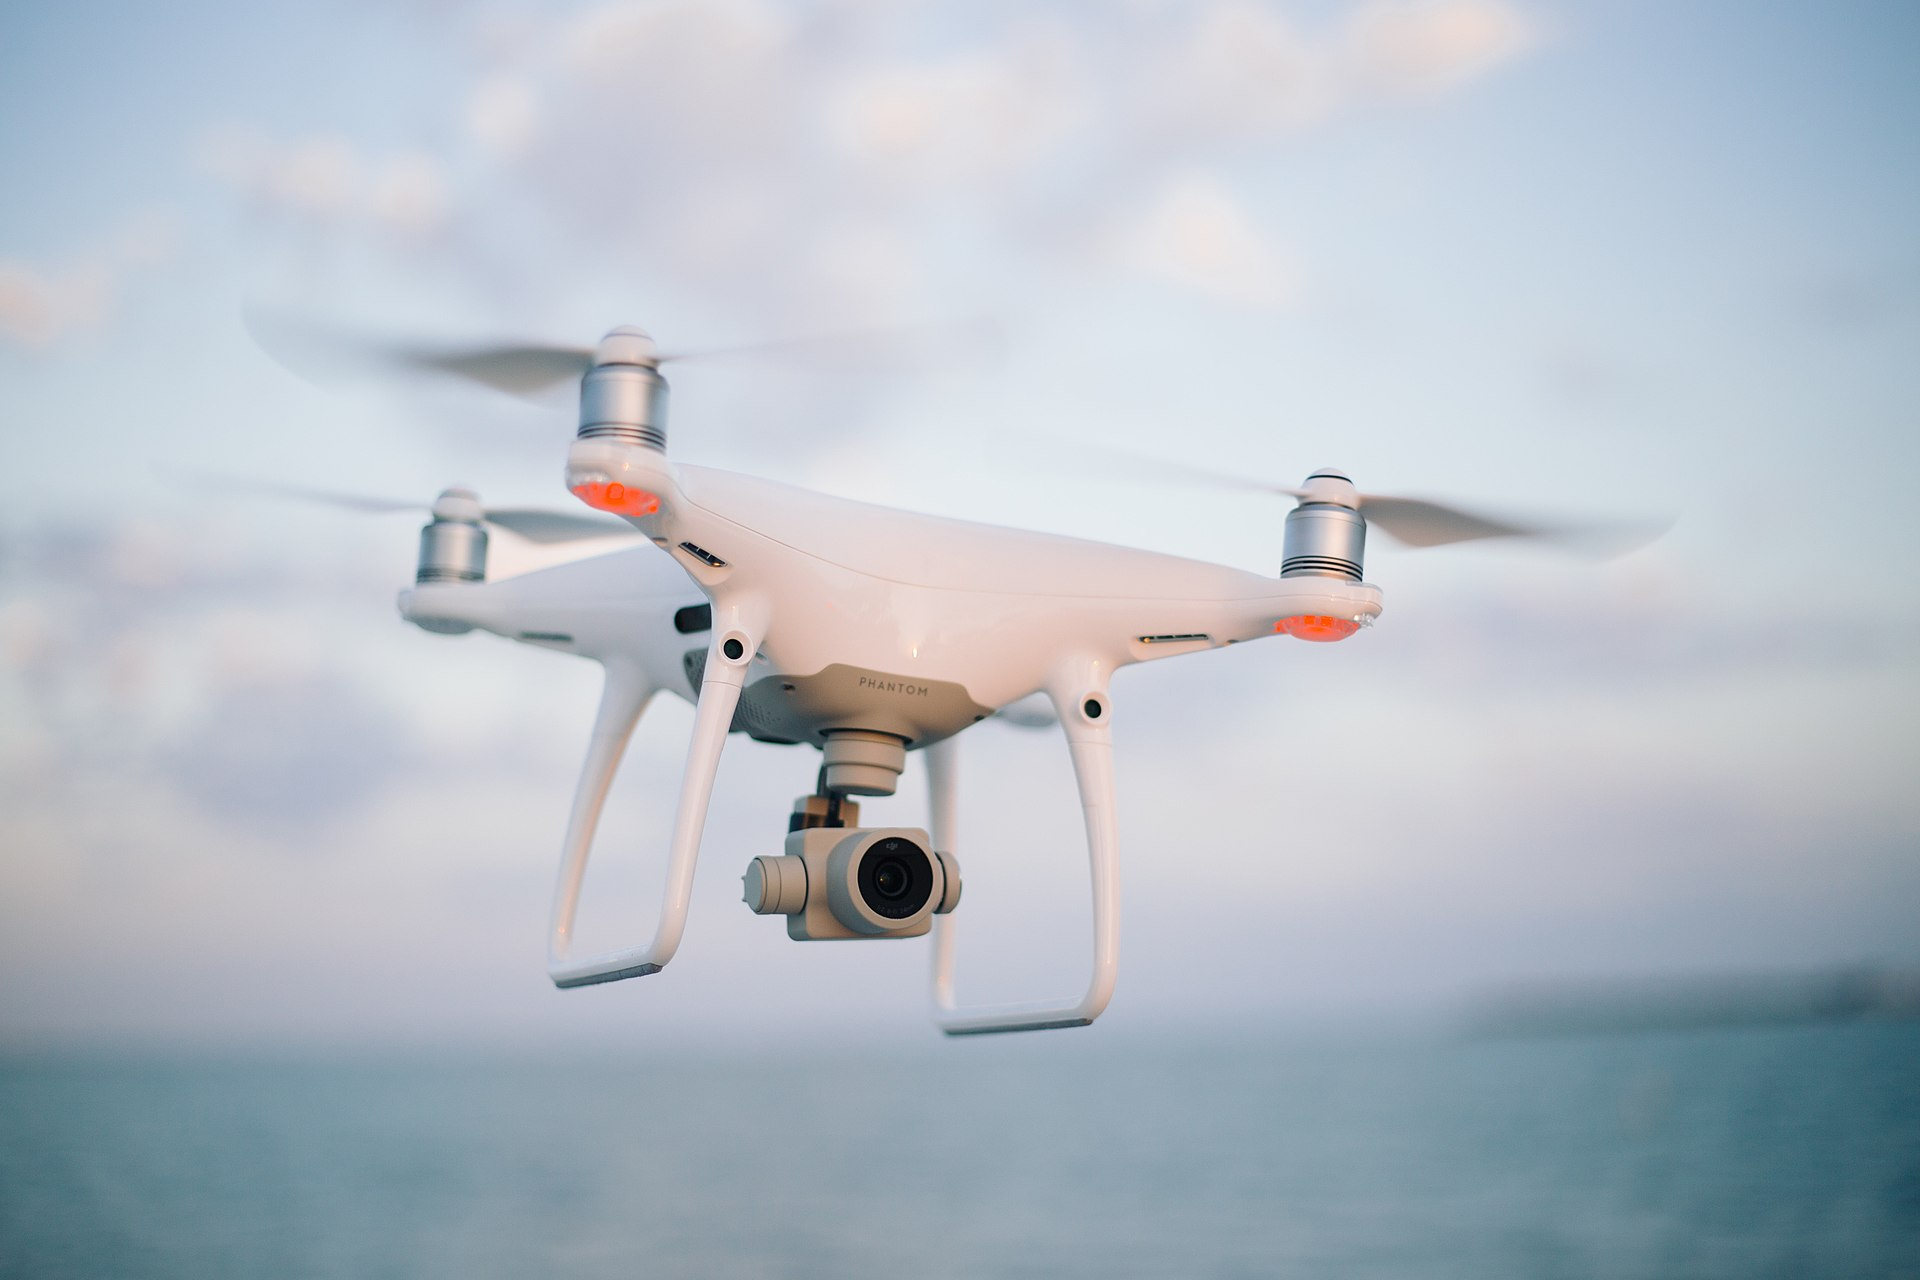
\includegraphics[width=\textwidth]{Images/Introduction/drone}
         \caption[Caption for LOF]{A DJI Phantom quadcopter (UAV)\protect\footnotemark}
         \label{fig:drone}
     \end{subfigure}
     \hfill
     \begin{subfigure}[b]{0.45\textwidth}
         \centering
         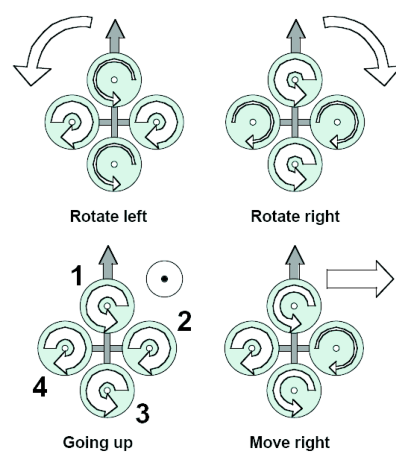
\includegraphics[width=0.6\textwidth]{Images/Introduction/propeller_direction.svg}
         \caption{Representation of the concept of a quadrotor. The width of the arrows is proportional to the angular speed of the propellers.\cite{Bouabdalla2007}}
         \label{fig:propeller_directions}
     \end{subfigure}
        \caption{A commercial quadrtotor platform with a representation of the quadrotor concept.}
        \label{fig:three graphs}
\end{figure}

\noindent The distinctive mechanical design of the quadrotor permits the actuation system to control all of the six degrees of freedom even though it is under-actuated. This is due to the fact that the rotational and translational dynamics are tightly coupled. Thus, all the translational and rotational motions can be carried off by properly controlling the magnitude and direction of the spinning speed of the rotors.   

\noindent \footnotetext[1]{\url{https://en.wikipedia.org/wiki/Quadcopter\#/media/File:Quadcopter_camera_drone_in_flight.jpg}, accessed on 01/08/2021.}


\pagebreak

Over the last few years, quadrotors have gained a large popularity in academia and in the industry. This is due to several reasons, such as: 

\begin{enumerate}

    \item Quadrotors are very simple to design and they can be easily assembled using relatively cheap components.  
    \item As quadrotors became more and more affordable and dependable, the number of real-world applications for quadrotors  has grown significantly. They are being used for aerial photography, agriculture, surveillance, inspection tasks, in addition to many other uses as well. 
    \item Quadrotors are quite agile and maneuverable during flight, especially when compared to other types of UAVs.
    
\end{enumerate}

However, one of the main challenges in the quadrotors community is the capability to design control and planning methods that will allow the quadrotors to carry out aggressive maneuvers.  The fast dynamics associated with typically small dimensions of such agile quadrotors, along with several aerodynamic effects that will become crucial during aggressive flight maneuvers, are just a few of the main problems that are faced during the system control design. Moreover, accurate tracking of the provided trajectory is a big issue in the case of aggressive maneuvers when the rotors are commanded high speeds and accelerations, which will cause rotors to become saturated and may also cause delays.


 \section*{Parallel manipulators}

A parallel manipulator is a mechanical system that consists of two connected platforms, the fixed platform and the moving platform. The latter is linked to the fixed platform thanks to at least two serial chains that are working in parallel. When compared to serial manipulators, parallel manipulators are more accurate and rigid. In addition, the ability to install the motors next to the fixed platform is a very important feature for them. Moreover, parallel manipulators can be used in a wide variety of applications that demand precision and high payload combined with high speed.\cite{Parallel_Manipulators}

\begin{figure}[h]
     \centering
     \begin{subfigure}[h]{0.45\textwidth}
         \centering
         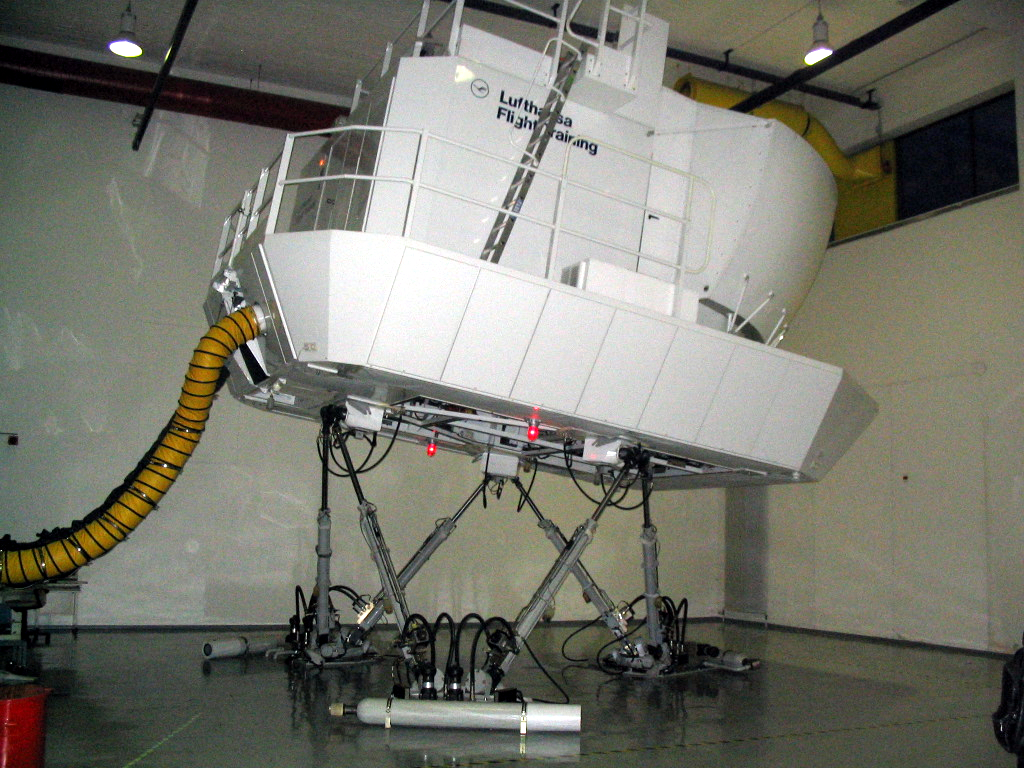
\includegraphics[width=0.7\textwidth]{Images/Introduction/GS}
    \caption[Caption for LOF]{Gough-Stewart used for a flight-simulator application.\protect\footnotemark}
         \label{GS}
     \end{subfigure}
     \hfill
     \begin{subfigure}[h]{0.45\textwidth}
         \centering
         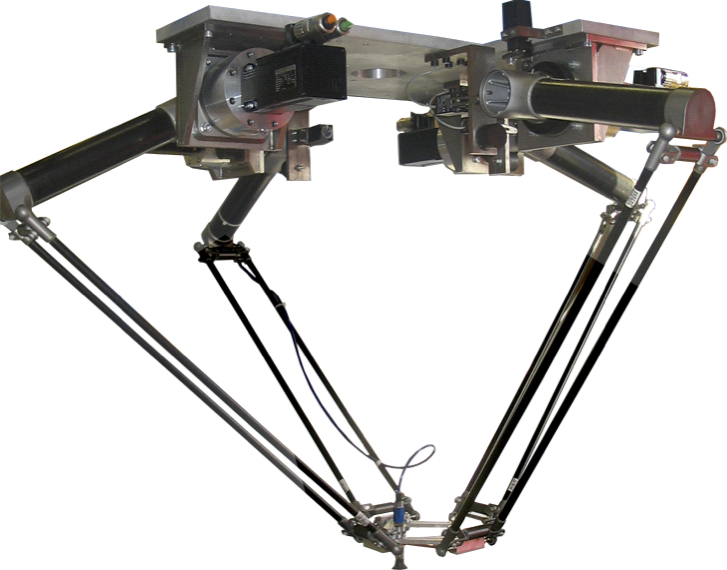
\includegraphics[width=0.7\textwidth]{Images/Introduction/PAR4}
         \caption[Caption for LOF]{The "PAR4" 4 degrees of freedom, high-speed, parallel robot prototype.\protect\footnotemark}
         \label{PAR4}
     \end{subfigure}
        \caption{Two examples of parallel robots.}
        \label{fig:three graphs}
\end{figure}




\footnotetext[1]{\url{https://en.wikipedia.org/wiki/Stewart_platform\#/media/File:Simulator-flight-compartment.jpeg}, accessed on 01/08/2021.}
\footnotetext[2]{\url{https://en.wikipedia.org/wiki/Parallel_manipulator\#/media/File:Prototype_robot_parall\%C3\%A8le_PAR4.jpg}, accessed on 01/08/2021.}


\pagebreak

However, parallel manipulators are subject to singularities which can lead to big problems in the robot workspace in case they were not handled correctly. Thus, the study of the singular configuartions of parallel manipulators is very important. Because, even just before reaching a singularity, the performance of the parallel manipulator will decrease dramatically. Moreover, the robot may loose the ability of moving in a certain direction, gain uncontrollable motions and the mechanism could even break. The main difference between serial and parallel manipulators is that singularity configurations may also appear inside the workspace of the robot (depending on the dimensions of the robot) and not just at the boundaries of the robot workspace, which can significantly decrease the area of the robot workspace.
As a result, many works have been developed by robotics researchers in order to allow parallel manipulators to safely cross these singularities by using trajectory planning and specific control methods.

\section*{The goal of this thesis}

This master thesis lies at the intersection of parallel robotics and aerial robotics. The two fields may seem very different from each other. However, quadrotors can be seen as a particular case of a parallel manipulator. 
In fact, a parallel manipulator is made up of a wrench system, applied by the robot limbs on the moving platform. And, this wrench system will define the motion of the moving platform. In the same manner, each propeller in a quadrotor can be considered as a limb of a parallel robot and the moving platform to be controlled can be considered as the body of the drone. 
Specifically, the goal of this master thesis is to study a distinct class of aggressive maneuvers for quadrotors, namely flip maneuvers. By doing flip maneuvers, full rotations around one or more axes of the body of the quadrotor can be done. In addition, the quadrotor should also be able to perform the flip maneuvers in constrained environments.

\begin{figure}[h]
     \centering
     \begin{subfigure}[h]{0.45\textwidth}
         \centering
         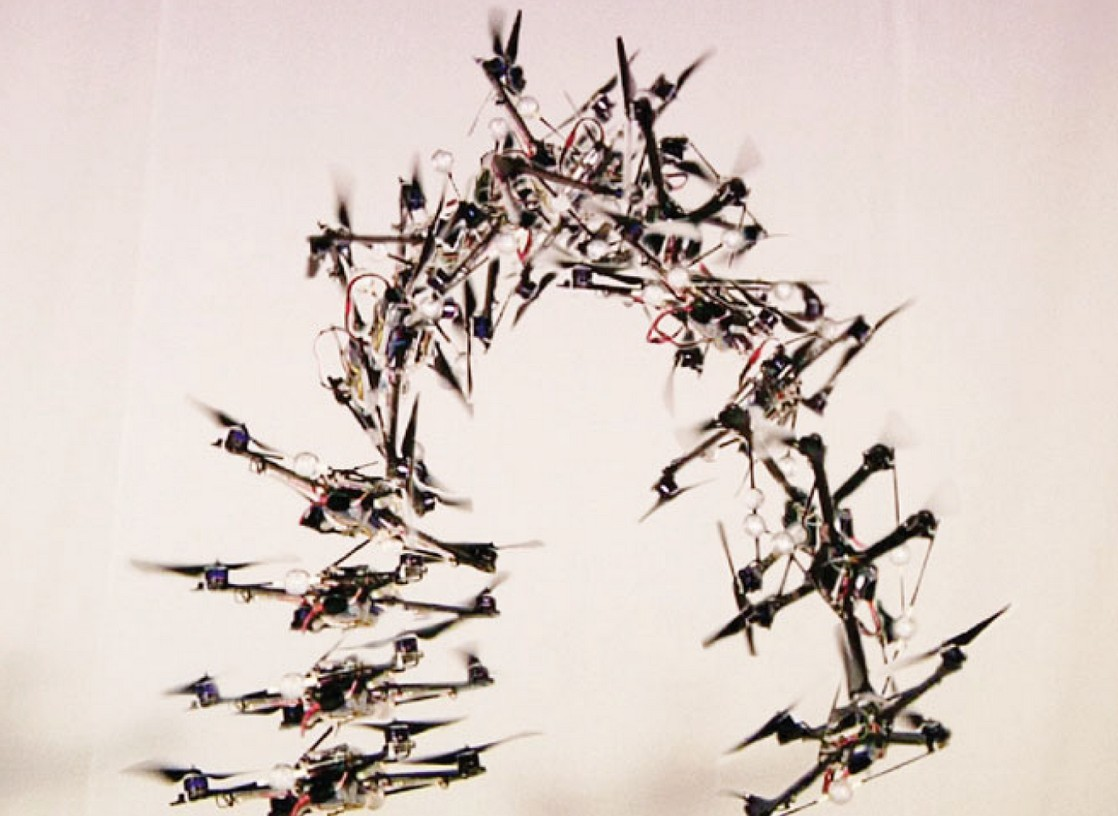
\includegraphics[width=0.9\textwidth]{Images/Introduction/flip}
    \caption{Quadrotor performing a triple flip.\cite{DAndrea2012}}
         \label{triple_flip}
     \end{subfigure}
     \hfill
     \begin{subfigure}[h]{0.45\textwidth}
         \centering
         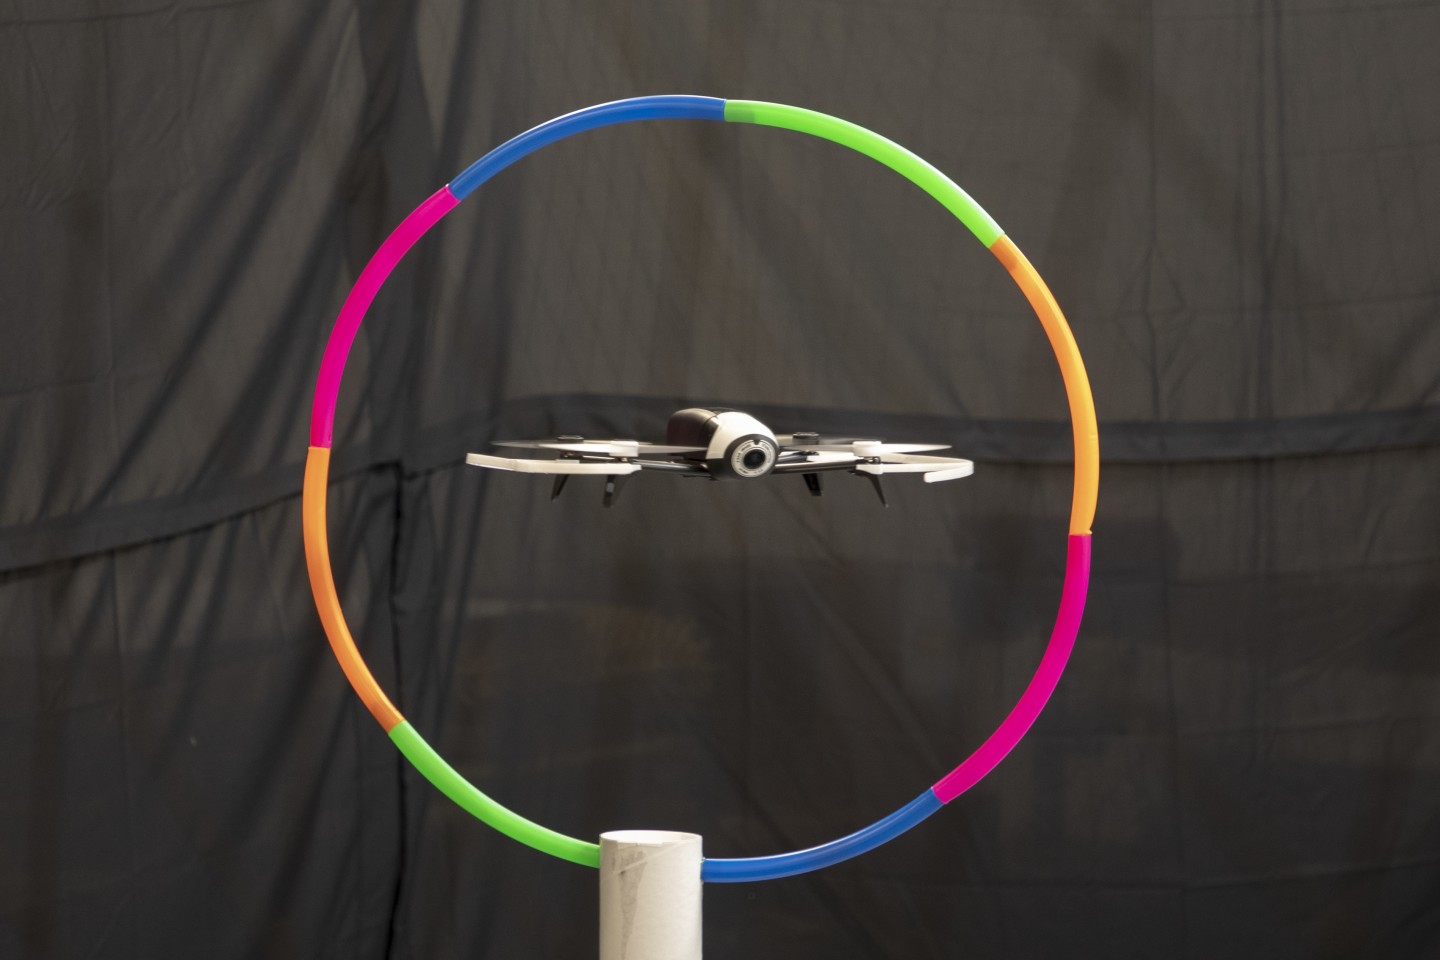
\includegraphics[width=\textwidth]{Images/Introduction/constrained_environment}
         \caption[Caption for LOF]{Quadrotor going though a loop.\protect\footnotemark[1]}
         \label{drone_hulahoop}
     \end{subfigure}
        \caption{Representation of the issues to be tackled in the master thesis.}
        \label{fig:three graphs}
\end{figure}

\footnotetext[1]{\url{https://newatlas.com/drones/muscle-signals-drone-control/\#gallery:2}, accessed on 01/08/2021.}

\pagebreak

\section*{Outline of the work}

The rest of the report is structured as follows:

\begin{comment}
\begin{itemize}
\setlength{\itemindent}{-.5in}
	\item [] \textbf{Chapter 1} is devoted to introduce the system modeling of quadrotors. Specifically, a simplified dynamic model of the quadrotor will be presented by using Euler-Lagrange formalism. Then, moving on from the simple dynamic model, a more detailed dynamic model will be presented by using the Newton-Euler formalism. Finally, the state-space model of the quadrotor will be derived.

	\item [] \textbf{Chapter 2} provides an overview of state of the art in quadrotor control in addition to introducing the different potential control methods that can be used during the master thesis in order to properly control the quadrotor. 

	\item [] \textbf{Chapter 3} provides detailed explanations of how multi-flip maneuvers can be handled. Then, the link between a quadrotor performing a flip and a parallel robot crossing a singularity will be explained. In the end, a literature review is provided in order to show how the problem is tackled by different researches.

	\item [] \textbf{Chapter 4} is devoted to trajectory optimization. By using trajectory optimization, it will be possible to create feasible trajectories for quadrotors to perform the aggressive maneuvers in constrained environments.
	
\end{itemize}
\end{comment}

\begin{itemize}
\setlength{\itemindent}{-.5in}
	\item [] \textbf{Chapter 1} provides an overview of the state of the art in the control of quadrotors and will later on focus on the main control method that will be used, namely Model Predictive Control (MPC). Moreover, a literature review of MPC applications on quadrotors will be presented. Furthermore, an overview on the software used to design a MPC controller will be presented. Finally, the state of the art in flipping maneuvers will be presented.
	
	 \item [] \textbf{Chapter 2} provides a detailed explanation of the quadrotor dynamics for the planar (2D) and 3D quadrotors. Morever, an Extended Kalman Filter (EKF) is then designed for the planar quadrotor case to be used in the presence of noisy measurements (states) and noisy control inputs. Finally, simulation results using MPC to reach a single waypoint and to follow circular trajectories with and without noise are presented.
	 
	 \item [] \textbf{Chapter 3} focuses on the trajectory generation of a flip trajectory where different optimization problems with different objective functions and initial conditions will be used in order to find the optimal flipping trajectory that satisfies the dynamic constraints of the quadrotor which will be used in the experimentation phase. Moreover, simulations with a MPC are then performed using the optimal flip trajectory.
	 
	 \item [] \textbf{Chapter 4} focuses on the simulations that were performed using ROS2 and Gazebo, in addition to the experimentation results.
\end{itemize}


\newpage
 
 \chapter{State of the art}
 
 In the following sections of this chapter, differential flatness,  the general control architecture of a quadrotor, different potential control approaches (linear and nonlinear), and the main control method that will be used to control a quadrotor, namely Model Predictive Control (MPC) will be explained. 
 \section{Differential Flatness}\label{Differential_flatness}  
 
 In the quadrotor community, a well-established finding is that the dynamic model of a quadrotor is differentially flat. Moreover, the control design problem in nonlinear systems will be considerably simplified. Precisely, a system with state $\textbf{\textsc{x}} \in \mathbb{R}^n$ and input $\textbf{\textsc{u}} \in \mathbb{R}^m$ is considered to be \textit{differentially flat} if there exists a set of \textit{flat outputs} $\textbf{\textsc{y}} \in \mathbb{R}^m$ which have the following form:
 
 \begin{equation}
 \textbf{\textsc{y}} = \textbf{\textsc{y}}(\textbf{\textsc{x}}, \textbf{\textsc{u}}, \dot{\textbf{\textsc{u}}},...,\textbf{\textsc{u}}^{(p)})
 \end{equation}

 With, 
 
 \begin{equation}
 	\begin{cases}
 		\textbf{\textsc{x}} = \textbf{\textsc{x}}(\textbf{\textsc{y}}, \dot{\textbf{\textsc{y}}},...,\textbf{\textsc{y}}^{(q)}) \\
 	\\
 		\textbf{\textsc{u}} = \textbf{\textsc{u}}(\textbf{\textsc{y}}, \dot{\textbf{\textsc{y}}},...,\textbf{\textsc{y}}^{(r)}) \\
 	\end{cases}
 \end{equation}

 As a result, the new set of variables is required to be a function of the state, the input and the derivatives of the input. Moreover, this set should also have the same dimensions as the control input. In this manner, it is possible to rewrite both the state and the input in function of the flat outputs and the derivatives of the flat outputs. This is a very useful property in underactuated systems where $m<n$, such as quadrotors, because, it will allow to generate trajectories in the lower dimensional space $m$, then this trajectory will be mapped into the full dimensional space $n$. An example of this is shown in figure \ref{fig:differential_flatness} below:
 
 \begin{figure}
 	\centering
 	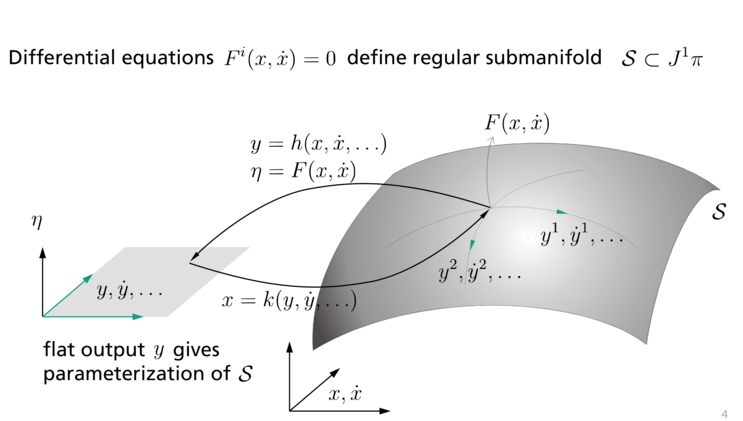
\includegraphics[width=0.7\textwidth]{Images/Control/differential_flatness.png}
 	\caption{Mapping between different dimensional spaces as a result of differential flatness. \cite{Fritzsche2019}}
 	\label{fig:differential_flatness}
 \end{figure}
 
 \newpage
 
 Another well known example of systems is a car, in which the underactuation is the result of the nonholonomic constraints that are imposed by the wheels. So, for a car, a generated trajectory for $(x,y)$ position of the rear-wheels is enough to specify all the viable trajectories of the system. Formal proofs that the quadrotor system is differentially flat can be found in \cite{Mellinger2011}, and \cite{Faessler2018} for the full model with first-order aerodynamics. The standard choice of flat outputs for the quadrotor is the coodinates of the center of mass and the yaw angle:

\begin{equation}\label{flat_outputs}
\textbf{\textsc{y}} = \begin{bmatrix}
x && y && z && \psi \\
\end{bmatrix}^{\intercal}
\end{equation}

Consequently, the problem of generating a feasible trajectory for a quadrotor then tracking it can be dimensionally decreased from a 6-dimensional space to a 4-dimensional space. By reason of the tight coupling between the rotational and translational dynamics, then defining a trajectory in function of the flat outputs $\textbf{\textsc{y}}$ is sufficient to properly define the full dynamics $\textbf{\textsc{x}}$.


\newpage

\section{General Control Architecture}
 Recently, many researchers have developed interest in the control of quadrotors. As a result, various control approaches have been proposed. The most known control architecture \cite{Faessler2018} consists of three nested control loops, as shown in figure \ref{fig:cascaded_pid_controller}, in order to generate the suitable motor commands to follow the desired signal. This controller is known as the cascaded controller. This strategy assumes that the attitude dynamics of a quadrotor are much faster than the translational dynamics. 
\begin{comment} 
Assuming that Euler angles are used to define the attitude and that a navigation module generates the desired trajectory $(\bm{r}_d(t),\psi_d(t))$ as shown in section \ref{Differential_flatness}, then:
 
\begin{itemize}
	\setlength{\itemindent}{-.5in}
	\item [] \textbf{Position controller} has the objective of driving the errors occurring on the translational dynamics to zero.
		And, the outputs of this outer loop are the thrust $f=u_1$, which is sent to the motor controller, and the desired attitude $(\theta_d(t),\phi_d(t))$, which corresponds to the reference signal of the attitude controller.
	\item [] \textbf{Attitude controller} has the goal of driving the errors occurring on the rotational dynamics to zero. This controller generates the inputs 
	$\bm{\tau}=\begin{bmatrix}
	u_2 && u_3 && u_4 \\
	\end{bmatrix}^{\intercal}
	$
	that are then sent to the motor controller.
	\item [] \textbf{Motor controller} This controller receives the control inputs 	$\bm{u}=\begin{bmatrix}
	f && \bm{\tau}
	\end{bmatrix}^{\intercal}
	$ and maps them into the desired spinning velocities $\Omega_i$ for each individual rotor. Moreover, low-level control laws are designed and realized in the firmware of the drone to make the convergence from the actual rotations to these desired values.
\end{itemize}
 

 
 \begin{figure}[h]
 \centering
 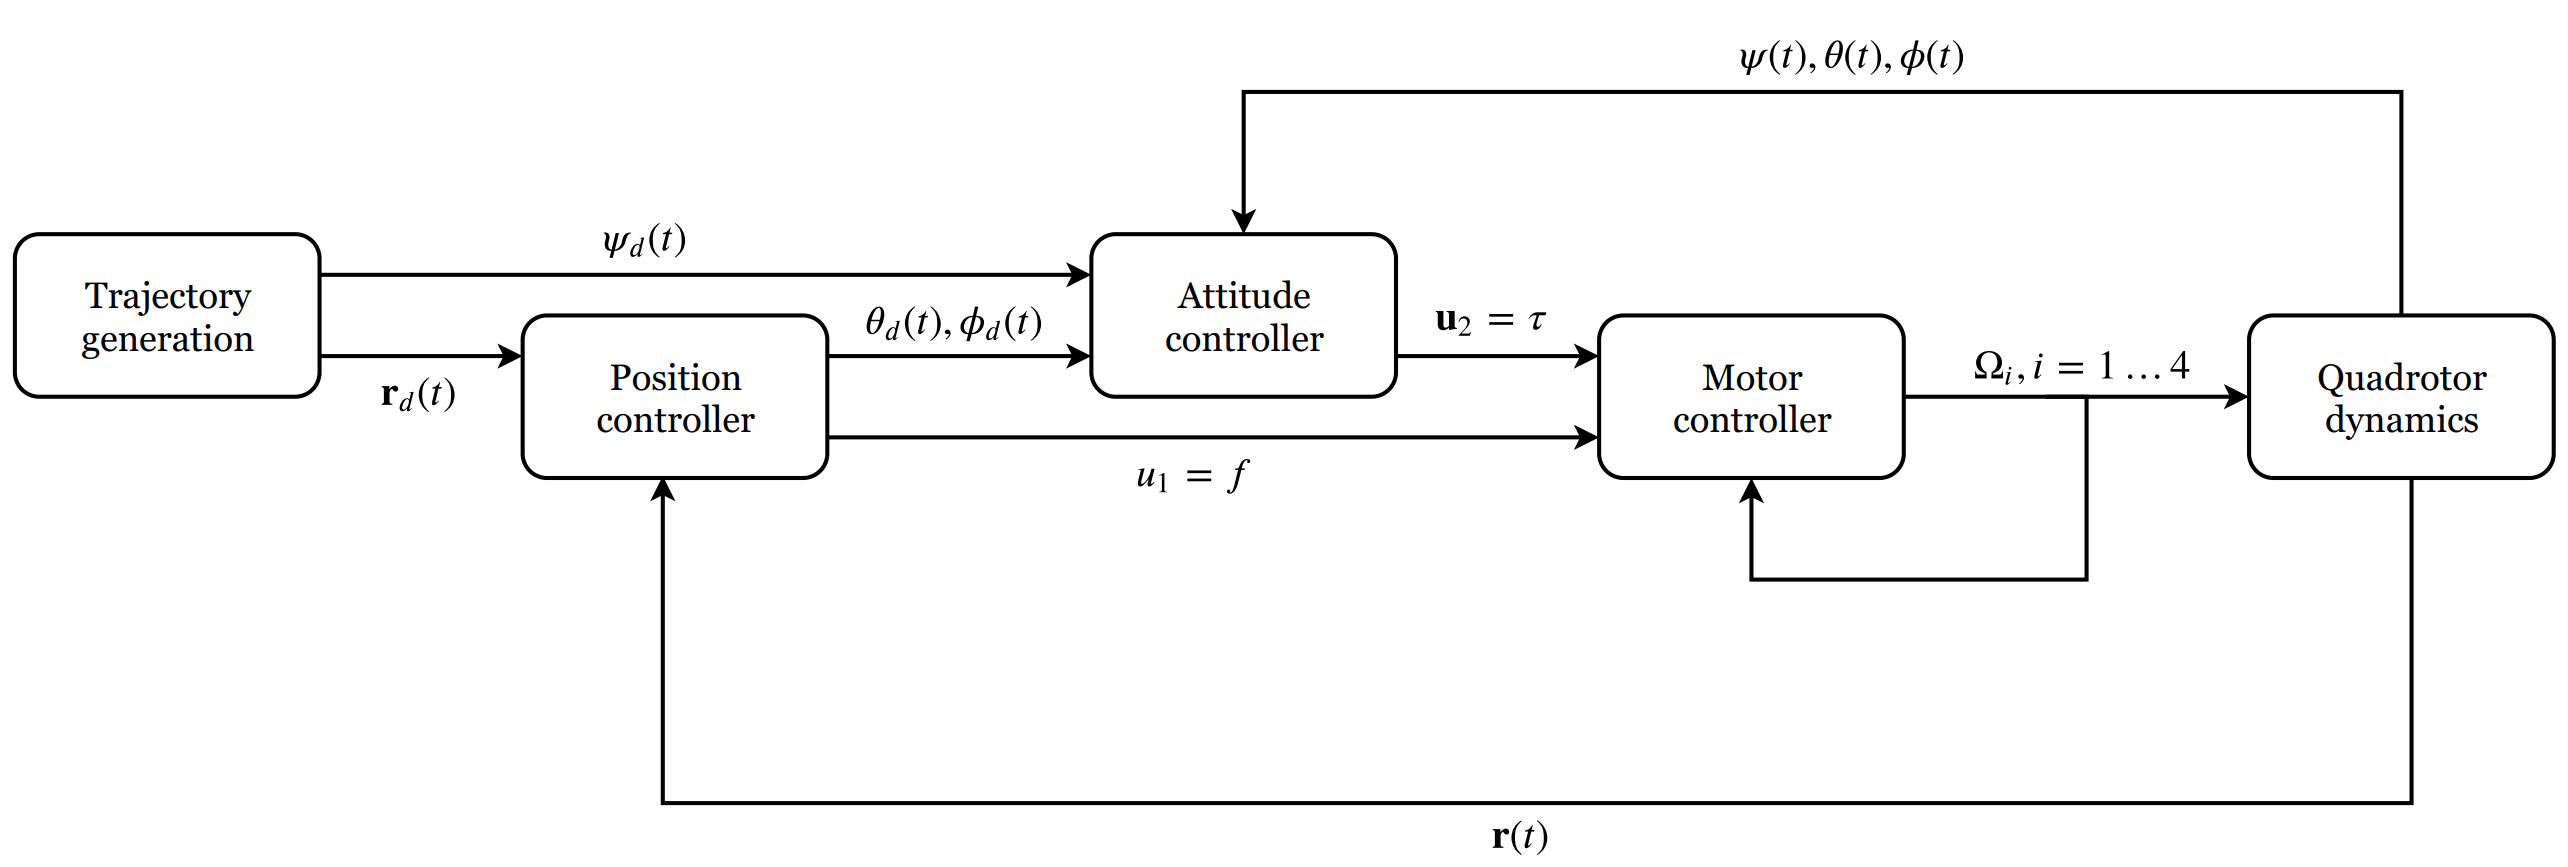
\includegraphics[width=0.8\textwidth]{Images/Control/General_control_architecture}
 \caption{Cascaded controller architecture.}
 \label{General_control_architecture}
 \end{figure}
 
There also exists different implementations of the cascaded controller that was shown in figure \ref{General_control_architecture}. An example of another architecture of a cascaded controller is shown below: 

\end{comment}



\begin{figure}[h]
	\centering
	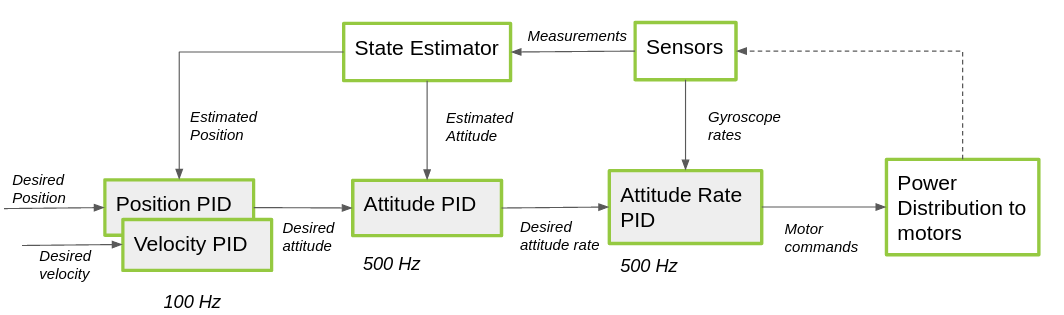
\includegraphics[width=\textwidth]{Images/Control/cascaded_pid_controller.png}
	\caption{Cascaded PID controller that is present on the crazyflie 2.1 quadrotor \cite{bitcraze}.}
	\label{fig:cascaded_pid_controller}
\end{figure}

In this case, the position and velocity controller, attitude controller and attitude rate controller are all PID controllers. And, it is evident that the attitude dynamics (who's attitude and attitude rate controllers operate at a frequency of 500Hz) are considered to be much faster than the translational dynamics (who's position and velocity controllers operate at a frequency of 100Hz). Moreover, 

\begin{itemize}
	\setlength{\itemindent}{-.5in}
	\item [] \textbf{Attitude Rate PID controller} directly controls the attitude rate. It receives the gyroscope rates after they have been filtered and uses the error between the desired attitude rate and current attitude rate, and outputs the motor commands which are then directly sent to the power distribution.
	
	\item [] \textbf{Attitude PID controller} directly controls the attitude of the drone. It takes the estimated attitude from the state estimator and uses the error between the desired attitude and the current attitude to output the desired attitude rate.
	
	\item [] \textbf{Position and Velocity PID controller} is the most outerloop of the cascaded PID controller. It receives the position or the velocity input from the high level commander which are then handled to output the desired attitude.
	 
\end{itemize}

 \newpage 
\section{General Control Approaches}\label{control_approaches_for_multi_flip_maneuvers}

\subsection{Method of Linearization}

By using extreme assumptions, it is feasible to apply linear control techniques in order to control a quadrotor (\cite{Sabatino2015}, \cite{BouabdallahNothSiegwart2018}). Particularly, this can be made by doing a linearization of the full dynamic model around an equilibrium point $\overline{\textbf{\textsc{x}}}$ and by using the assumption that the vehicle is only capable of oscillating lightly around the hover point.
It is very easy to observe that a feasible equilibrium is provided by a configuration where the center of mass is at a random position $\overline{\textbf{\textsc{r}}}$ and all the other elements of the state are set to zero. So, the nominal input $ \textbf{\textsc{u}} = \overline{\textbf{\textsc{u}}}$ to sustain such equilibrium can be assessed as the thrust that is required to compensate the gravity force:

\begin{equation}
\overline{\textbf{\textsc{u}}} = \begin{bmatrix}
f \\ 
\bm{\tau}\\
\end{bmatrix}=
\begin{bmatrix}
mg \\
\bm{0_{3 \times 1}} \\
\end{bmatrix}
\end{equation}

At this stage, the complete non-linear dynamics that have the form :

\begin{equation}
\dot{\textbf{\textsc{x}}}=\overline{\textbf{\textsc{f}}}(\overline{\textbf{\textsc{x}}},\overline{\textbf{\textsc{u}}})
\end{equation}

can now be linearized around the hover point $(\overline{\textbf{\textsc{x}}},\overline{\textbf{\textsc{u}}})$ as shown below.

\begin{equation}
\dot{\textbf{\textsc{x}}} = \begin{bmatrix}
\frac{\partial \textbf{\textsc{f}}(\textbf{\textsc{x}},\textbf{\textsc{u}})}{\partial \textbf{\textsc{x}}}
\end{bmatrix}_{(\bar{\textbf{\textsc{x}}},\bar{\textbf{\textsc{u}}})} \textbf{\textsc{x}}+ 
\begin{bmatrix}
\frac{\partial \textbf{\textsc{f}}(\textbf{\textsc{x}},\textbf{\textsc{u}})}{\partial \textbf{\textsc{x}}}
\end{bmatrix}_{(\bar{\textbf{\textsc{x}}},\bar{\textbf{\textsc{u}}})} \textbf{\textsc{u}} = \textbf{\textsc{A}}\textbf{\textsc{x}} + \textbf{\textsc{B}} \textbf{\textsc{u}}
\end{equation}

It can be demonstrated that both matrices $\textbf{\textsc{A}}$ and $\textbf{\textsc{B}}$ can be used to determine a linear system that is both controllable and observable \cite{Sabatino2015}. Thus, any control technique that is linear can now be used on the quadrotor in order to keep it around a desired equilibrium point, such as optimal LQR/LQG \cite{Cowling2007,Minh2010} control or simple PD or PID controller \cite{Han2012,Altug2007}.


 \subsection{Nonlinear Control Methods}
 

In order to perform more complex tasks and follow aggressive trajectories, nonlinear control methods are required.
A comprehensive literature review on this topic is beyond the scope of this work and several works can be found, such as \cite{Zulu2016}, which provides a general overview on nonlinear control of quadrotors. However,
some nonlinear control methods deserve to be mentioned due to their extensive use and applications:

\begin{itemize}
\setlength{\itemindent}{-.5in}

	\item [] \textbf{Sliding Mode control} It is a control technique that is nonlinear presenting exceptional attributes of robustness,accuracy, easy tuning and execution. The aim of SMC systems is to drive the system states to a specific surface in the state space, called  \textit{"sliding surface"}. Upon reaching the sliding surface, sliding mode control allows the states to remain on the close neighborhood of the sliding surface. Therefore, the sliding mode control consists of a controller design with two parts. The first part contains the design of a sliding surface in order for the sliding motion to fulfill design requirements. The second deals with selecting a control law that makes the switching surface interesting with respect to the system state \cite{Utkin1997}.
There exist two main benefits of sliding mode control. Firstly, the behavior of the dynamics of the system can be changed according to a specific selection of the sliding function. Secondly, the response of the closed loop system becomes completely insensitive to some special uncertainties. This principle goes beyond bounded model parameter uncertainties, interference and non-linearity. In a practical sense, SMC allows the control of nonlinear processes that are affected by external noise and heavy model uncertainties.
The most important principles of SMC are shown in the following significant references \cite{Utkin1997,DeCarlo1998,Hung1993}. Researchers have also studied the problems appearing in the practical execution of this class of techniques. \cite{Young1999}
Interested readers can refer to the book \cite{Bartolini2008} which presents a very modern overview of the most promising current line of theoretical and practical research in the domain.

	\item [] \textbf{Backstepping control} The main idea is to divide the system into successive subsystems and to apply a recursive algorithm which will stabilize each subsystem after the other \cite{Madani2006}. However, this method is not robust, but it is computationally fast. In order to handle disturbances, Fang et al. \cite{Gao2011} implemented an integral backstepping control law, in which the integral term was shown to reduce steady state errors and the response time of the system greatly. 

	\item [] \textbf{Adaptive control} This method is required when the parameters that are characterizing the system contain errors or are unknown. This type of control algorithms contains a parameter adaptation law, which is enclosed in the control to track the desired trajectory of the system, even if the model of the system is not completely known.
For instance, Diao et al. \cite{Diao2011} obtained good performance even though the inertial parameters of the quadrotor and the aerodynamic coefficients were not perfectly known. This method is convenient in some cases, such as the existence of unpredictable wind \cite{Antonelli2013} or pick-and-place applications with small loads. 
	 
 \end{itemize}
 

In the next section, the main control method that will be used in the master thesis will be explained.

\newpage

\section{Model Predictive Control}

\subsection{General Idea}\label{MPC_General_Idea}
 
 There exist "open-loop" methods \cite{Kirillova2000} in which the control input sequence $\textbf{\textsc{u}}(t)$ is designed using a model of the system and a set of constraints. However, the problem with this approach is that modeling errors and noise are not taken into consideration. So, these inputs will not necessarily generate the desired response from the system. Because of that, a \textit{"closed-loop"} strategy is required in order to cancel out these errors. So, an approach that can be used is called \textit{"Model Predictive Control"} (MPC). This method is also known as \textit{"receding horizon control"} \cite{How2008} because the \textit{"prediction horizon"} (which is a finite horizon) translates forward by one time step after the current optimization problem is solved . In short, MPC is a \textit{feedback control} algorithm which uses a model of the system to predict the future outputs of the system and it solves an optimization problem on-line in order to select an optimal control.
 
 \paragraph{Basic strategy}

The basic strategy of MPC is the following:


\begin{itemize}
	\item At time step $k$, the system model and an optimizer will be used in order to design a sequence of control inputs
	
	$$ \textbf{\textsc{u}}(k|k), \textbf{\textsc{u}}(k+1|k), \textbf{\textsc{u}}(k+2|k), \textbf{\textsc{u}}(k+3|k),...,\textbf{\textsc{u}}(k+N|k) $$
	
	starting from the current state $\textbf{\textsc{x}}(k)$ over a prediction horizon $N$.
	\item Only the first step of the sequence of control inputs will be applied on the system.
	\item The processes above are then iterated for time $(k+1)$ at state $\textbf{\textsc{x}}(k+1)$. 
\end{itemize}
 
 
 \begin{figure}[h]
 \centering
 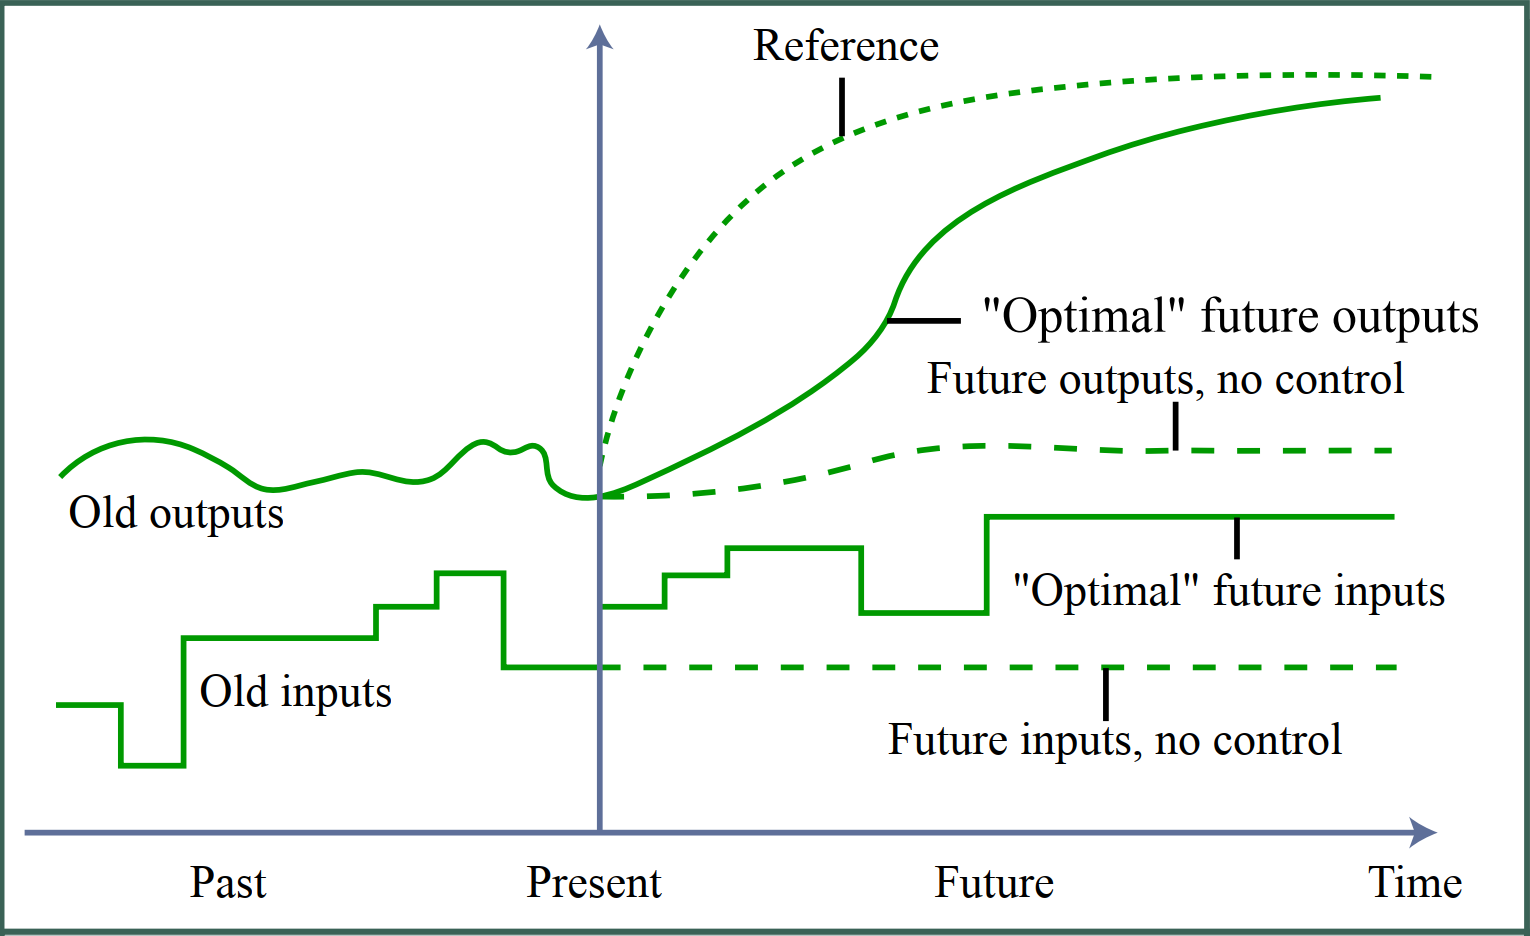
\includegraphics[width=0.6\textwidth]{Images/Control/MPC_general_idea.png}
 \caption{Basic idea of MPC \cite{How2008}.}
 \label{MPC_basic_idea}
\end{figure}  
 
\noindent It should be noted that the control algorithm of MPC is based on numerically solving an optimization problem at each time step. And, it is a constrained optimization in general.
 
 \paragraph{Advantages and drawbacks of MPC} There are several advantages when using MPC: 
 
 \begin{itemize}
 	\item MPC is able to control multi-input multi-output (MIMO) systems which might have interactions between their inputs and outputs.
 	\item MPC explicitly accounts for the constraints that are imposed on the system. So, it does not just design a controller to keep the system away from the constraints.
 	\item MPC can easily handle nonlinear dynamics and time-varying plant dynamics, because the controller is explicitly a function of the model of the system which can be modified in real-time.
 \end{itemize}

\noindent The main drawback of MPC is that it usually requires a powerful and fast processor with a large memory in order to properly solve the problem at hand. This is because MPC solves an optimization problem at each time step.
 
\noindent There have been many commercial applications of MPC starting from the early 1970s in the process industry. The table \ref{table_MPC} below shows the different companies that have used MPC in different industries in 2014.
 

\begin{table}[h]
\setlength{\tabcolsep}{15pt} % Default value: 6pt
\renewcommand{\arraystretch}{1} % Default value: 1
 \caption{The number of MPC applications in different industries in 2014 \cite{Kozak2014}.}
 \label{table_MPC}
\begin{tabular}{l c c c c c r}
Application & Aspen & Honeywell & Adersa & CCI & Pavilion & Total \\
\hline
Refining & 950 & 300 & 290 & - & 15 & 1555 \\
Chemicals & 437 & 55 & 12 & 21 & 25 & 550 \\
Food & - & - & 48 & - & 14 & 62 \\
Pulp paper & 21 & 39 & - & - & 3 & 63 \\
Gas and air & 11 & 13 & - & 24 & - & 48 \\
Polymer & 5 & - & - & - & 22 & 27 \\
Utilities & 7 & 9 & - & 6 & - & 22 \\
Other & 39 & - & 51 & 6 & - & 96 \\
\hline 
\hline
Total & 1470 & 416 & 401 & 57 & 79 & 2423 \\
\end{tabular}
\end{table}

\noindent However, as computational power has increased throughout the years thanks to the advancement of technology, there has been a renewed curiosity in applying this control approach to systems with fast dynamics for which the computational complexity is significantly larger when compared to the industrial applications for which computational complexity was not a concern (since MPC was applied on systems with slow dynamics in that case).
 
\subsection{Design Parameters}
The different parameters that can be tuned in a MPC controller (\cite{MathWorks2018, MathWorks2018b, MathWorks2018c}) are the following:

\begin{itemize}
	\item The sample time $T_s$.
	\item The prediction horizon $N$.
	\item The control horizon $m$.
	\item The constraints.
	\item The weights.
\end{itemize}

\noindent Choosing the proper values for the parameters stated above is very important since they affect the performance of the controller and the computational complexity of the MPC algorithm.

\paragraph{Sample Time $T_s$} 

The sample time determines the rate at which the controller executes the control algorithm. \begin{itemize}
	\item If $T_s$ is too large, then when disturbances occur, the controller will be unable to react to the disturbances quickly enough.
	\item If $T_s$ is too small, the controller will have much faster reaction times to disturbances and set-point changes. However, this comes at the cost of an excessive computational load.
\end{itemize}

\noindent In order to find reasonable balance between controller performance and computational effort, the general recommendation is to have between 10\% and 25\% of the minimum desired closed-loop response time .

\paragraph{Prediction horizon $N$} 

The prediction horizon $N$ (sometimes referred to with the variable $p$, however, $N$ will be used instead for the remaining of this report) is the number of predicted future time steps of the system. It shows how far the controller predicts into the future. Thus, a prediction horizon must be chosen in such a way that it covers the significant dynamics of the system. However, it should be noted that a large prediction horizon should not be selected, since unexpected phenomenons could occur that may affect the dynamics of the system, which will cause a waste of computational power. The general recommendation is to increase $N$ until additional increases will have little impact on the performance. The maximum $N$ is the number of control intervals needed for the open-loop step response of the system to become infinite. However, having $N>50$ is hardly ever required unless $T_s$ is very small.

\paragraph{Control horizon m}

The control horizon is the set of future actions which will lead to the predicted plant output. It represents the number of control moves until time step $m$. After the first $m$ steps, the remaining inputs will remain constant as shown in figure \ref{MPC_basic_idea} for the \textit{"Optimal"} future inputs. Moreover, each control input element in the control horizon is a free variable that will be computed by the optimizer. Thus, the smaller the control horizon, the fewer the computations. However, setting $m=1$ may not give the best possible output for the system. And, similarly to the prediction horizon, if the control horizon is increased, this will lead to better predictions at the cost of increasing the computational complexity. Moreover, the general recommendation for the control horizon is to keep it much smaller than the prediction horizon, because:

\begin{itemize}
	\item A smaller control horizon $m$ will lead to less variables to optimize in the QP that will be solved at each control input interval. This will encourage quicker computation times.
	\item If delays are considered, then having $m<N$ is mandatory. Otherwise, some control input elements within the control horizon  may not have any effect on the plant outputs before the prediction horizon ends, which will lead to a QP Hessian matrix which is singular. 
	\item Having a small value for $m$ encourages having an internally stable controller. However, this is not guaranteed.
\end{itemize}

\paragraph{Constraints} A model predictive controller can integrate constraints on the inputs, the rate of change of the inputs and the outputs. In addition, the constraints can be \textit{"soft"} constraints or \textit{"hard"} constraints. \textit{"Soft"} constraints represent constraints that are allowed to be violated if the MPC deems it to be necessary in order to find a solution for the control problem at hand.
In addition, it should be noted that \textit{hard} constraints are a set of constraints that cannot be violated by the MPC. However, applying hard constraints on both the inputs and outputs at the same time may cause conflicts to occur between the constraints, which may lead to an unfeasible solution. Moreover, the general recommendation is to use soft constraints on the outputs and to avoid having hard constraints on both the inputs together with the rate of change of the inputs.

\paragraph{Weights} Model Predictive Control could have many goals. A possible goal could be to have the outputs converge to their set-points as fast as possible. Another goal could be to have smooth control inputs in order to avoid aggressive control maneuvers. So, in order to achieve a balanced performance between these two competing goals, the input rates and the outputs can be weighted relatively to each other. It is also possible to adjust relative weights within the input rates and the outputs.

\subsection{Basic formulation of a MPC problem} 

For a given set of plant dynamics which is first assumed to be linear:

\begin{equation}
\begin{cases}
\textbf{\textsc{x}}(k+1) = A\textbf{\textsc{x}}(k) + B \textbf{\textsc{u}}(k) \\
\textbf{\textsc{z}}(k) = C \textbf{\textsc{x}}(k)\\
\end{cases}
\end{equation}

\noindent and a cost function as follows: 

\begin{equation}
J = \sum_{j=0}^{N} \{ \|\textbf{\textsc{z}}(k+j|k)\|_{R_{zz}} + \|\textbf{\textsc{u}}(k+j|k)\|_{R_{uu}} \} + F \textbf{\textsc{x}}(k+N|k))
\end{equation}

 
\noindent With: 
 
 \begin{itemize}
 	\item $\|\textbf{\textsc{z}}(k+j|k)\|_{R_{zz}}$ is the weighted $L^2$-norm of the state, so it is expressed as follows:

 \begin{equation*}
 \|\textbf{\textsc{z}}(k+j|k)\|_{R_{zz}} = \textbf{\textsc{z}}(k+j|k)^{\intercal}R_{zz}\textbf{\textsc{z}}(k+j|k)
\end{equation*}   	
 	
	\item  	$\|\textbf{\textsc{u}}(k+j|k)\|_{R_{uu}}$ is the weighted $L^2$-norm of the control input sequence, so it is expressed as follows:
	
\begin{equation*}
 \|\textbf{\textsc{z}}(k+j|k)\|_{R_{zz}} = \textbf{\textsc{z}}(k+j|k)^{\intercal}R_{zz}\textbf{\textsc{z}}(k+j|k)
\end{equation*}  

	\item $F \textbf{\textsc{x}}(k+N|k))$ is a terminal cost function which can also have weights if required.
 	
\end{itemize}  
 
It should be noted that if  $N \rightarrow \infty$, and there are no additional constraints on  $\textbf{\textsc{z}}$ and/or $\textbf{\textsc{u}}$, then the problem falls back to the discrete LQR problem \cite{Kostova2013}. Moreover, when limits are added on 
  $\textbf{\textsc{x}}$ and/or $\textbf{\textsc{u}}$, then the general solution cannot be found anymore in analytical form, and it has to be solved numerically.

Furthermore, solving for a very long sequence of control inputs is irrelevant if the model used for the computations is expected to be erroneous or there are disturbances applied on the system, since only the first element of the optimized control sequence will be implemented. This is why MPC is generally designed by using a relatively small $N$.
  
  \paragraph{Typical problem statement}
  
  For a finite $N$ and with $F=0$ the problem can be expressed as follows: 
  
\begin{mini}|s|
{u}{ J = \sum_{j=0}^{N}{  \{ \|\textbf{\textsc{z}}(k+j|k)\|_{R_{zz}} + \|\textbf{\textsc{u}}(k+j|k)\|_{R_{uu}} \} }}
{}{}
\addConstraint{ \textbf{\textsc{x}}(k+j+1|k) = A\textbf{\textsc{x}}(k+j|k) + B \textbf{\textsc{u}}(k+j|k) }
\addConstraint{ \textbf{\textsc{x}}(k|k) \equiv \textbf{\textsc{x}}(k) }
\addConstraint{\textbf{\textsc{z}}(k) = C \textbf{\textsc{x}}(k+j|k)}
\addConstraint{|\textbf{\textsc{u}}(k+j|k)| \leq u_{max}}
{}
\label{optim_problem}
\end{mini}

\subsection{MPC applications on quadrotors}

 There have been numerous applications of MPC on quadrotors. The main MPC applications on drones can be separated into two different categories:

\subsubsection{Centralized MPC}
 
In this type of application, the MPC controller is a signle structure that encapsulates both the translational dynamics and the rotational dynamics. It takes the trajectory waypoints as inputs, and directly outputs the control inputs required to control the quadrotor. This type of implementation of the MPC controller produces the least amount of errors. However, this comes at a cost of a larger computational load.

\begin{figure}[h]
	\centering
	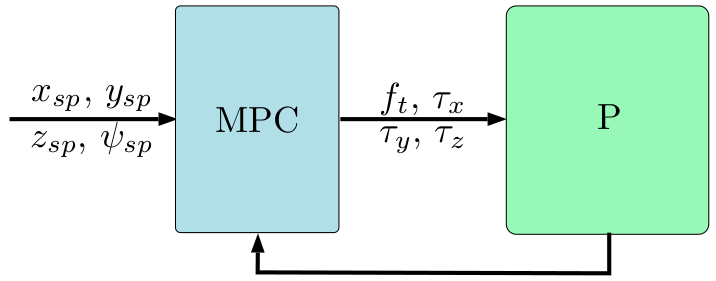
\includegraphics[width=0.7\textwidth]{Images/Control/MPC/centralized_mpc.png}
	\caption{Example of a centralized MPC control loop \cite{Alvarez-Valle2019}.}
	\label{fig:centralized_mpc}
\end{figure}

As can be seen in figure \ref{fig:centralized_mpc}, which represents a centralized control loop structure for a basic MPC, the right block is the plant which represents the quadrotor dynamics. The MPC bloc taks as input the desired trajectory, and outputs control inputs to allow the quadrotor to follow the trajectory.

It should be noted that different versions of the MPC controller shown in figure \ref{fig:centralized_mpc} can exist. For example, another version of the MPC could be that the state variables of roll and pitch angles can be added as outputs. This is mainly implemented in order to ensure that the quadrotor does not take extreme values in roll and pitch angles, which can potentially destabilize it, because no restrictions are being used for these angles otherwise.

\newpage

\subsubsection{Non-centralized MPC} 

In this type of application, the state-space of the system will be split to obtain two different controllers in a master-slave structure. This more simplified structure allows the implementation of MPC in different embedded systems, each one with less computational load when compared to the complete structure of a centralized MPC. For example, the simplified slave structure can be used to control the attitude of the quadrotor, whereas the master structure can be used to control the position and direction of the quadrotor. In addition, this splitting allows different sample times for the master and slave loops \cite{Bingfang2004}. Furthermore, an implementation of non-centralized MPC could be of having both master and slave structures being MPC controllers. An example of this non-centralized MPC implementation is shown in figure \ref{fig:non_centralized_mpc_1} below:

\begin{figure}[h]
	\centering
	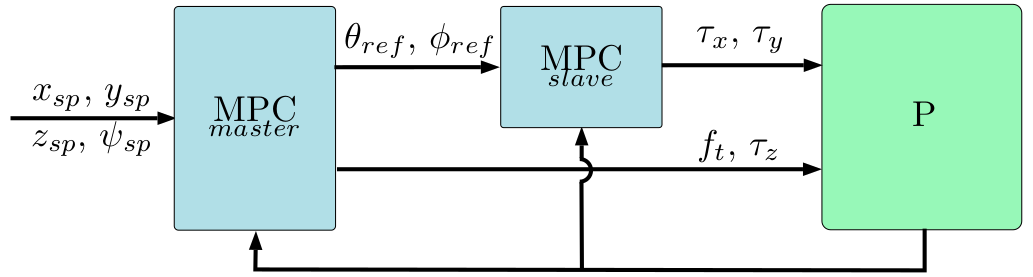
\includegraphics[width=0.9\textwidth]{Images/Control/MPC/non-centralized_mpc_1.png}
	\caption{Example of a non-centralized MPC-MPC control loop \cite{Alvarez-Valle2019}.}
	\label{fig:non_centralized_mpc_1}
\end{figure}

Another implementation is using a MPC controller for the master structure and pairing it with the slave structure that is using a controller with a different control law, such as a PD-P controller, in order to further reduce the computational load. An example of this non-centralized MPC implementation is shown in figure \ref{fig:non_centralized_mpc_2} below:

 \begin{figure}[h]
	\centering
	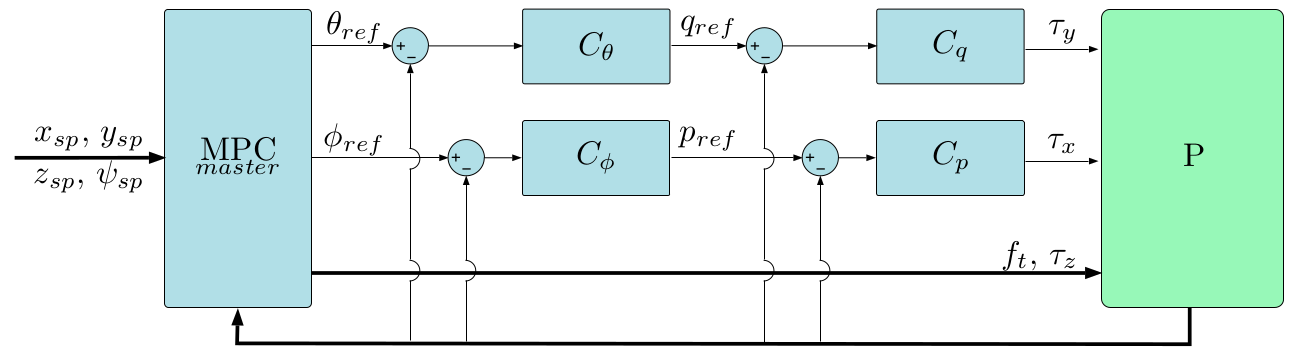
\includegraphics[width=0.9\textwidth]{Images/Control/MPC/non-centralized_mpc_2.png}
	\caption{Example of a non-centralized MPC-PD-P control loop \cite{Alvarez-Valle2019}.}
	\label{fig:non_centralized_mpc_2}
\end{figure}

However, since the control law in this master thesis will be entirely focused on MPC controllers, and since the task will be to follow aggressive trajectories as perfectly as possible, then the centralized MPC was chosen since it is the simplest implementation of MPC and it results in the least amount of errors when compared to non-centralized MPC implementations. In addition, the computational load of MPC will not be a problem, since the MPC controller will not be running on the quadrotor itself. All the computations will be done on a computer which will have considerably larger computational power than the processor of the quadrotor. And, the control inputs will be sent to the quadrotor via radio signals. However, it should be noted that the quadrotor will be susceptible to delays.

In the next section, the software used to implement the MPC controller is presented.

 \newpage  
	 

 
 \section{acados – fast embedded optimal control solvers}
 
 \subsection{The difference between acados and other embedded optimal control solvers}
 A big role in bringing MPC to real-time applications is played by the implementation of efficient embedded optimal control methods. This gave rise to software
packages such as:
    \begin{itemize}
        \item \texttt{MPT}: for explicit MPC \cite{MPT3}.
        \item \texttt{qpOASES}: an active-set solver for quadratic programming \cite{qpOASES}.
        \item \texttt{FORCES}: an interior-point solver for quadratically constrained QP and NLPs with optimal control structure \cite{FORCES}.
        \item \texttt{ACADO Code Generation tool}: for tailored SQP based NMPC solvers \cite{ACADO}.
    \end{itemize}

One challenge in developing software for embedded optimal control lies in the trade-off between flexibility, memory usage and speed. Moreover, many of the software packages mentioned above are based on \textit{automatic code generation}. This allows to have self-contained and efficient routines. However, the size of the problem and the choice of algorithms are usually fixed for one specific optimal control instance, which will result in a loss of flexibility. In addition, generated code is often hard to read, thus hard to debug. Finally, it is hard to predict if an automatic code optimization strategy is beneficial or counterproductive for some types of problems. This means that in some cases, a programmer can create faster and more efficient code.

For these reasons, \texttt{acados} does not rely on automatic code generation to perform linear algebra operations. Instead, the high-performance linear algebra package \texttt{BLASFEO} is used. 

Furthermore, other embedded optimal control softwares use global data in order to not sacrifice execution speed and memory. The resulting codebase is difficult to understand, maintain and extend. However, \texttt{acados} organizes the code in a modular way, with formal interfaces between the different algorithmic components. This makes it easier to interchange solvers, routines and libraries needed for the embedded control algorithm.

Finally, \texttt{acados} uses \texttt{CasADi} modeling language instead of \texttt{Mathematics}, \texttt{sympy} or \texttt{MATLAB Symbolic Toolbox}. Many of these softwares make use of expression trees to represent mathematical funcions, which could lead to a large code size, high memory usage and slow evaluation of high-order derivatives for non-trivial models. Whereas \texttt{CasADi} is based on expression graphs. This usually leads to smaller and faster code which make it more suitable for embedded applications. In addition, it is free and open-source software. In summary, \texttt{acados} offers the following:

\begin{itemize}
	\item It contains efficient optimal control algorithms implemented in C.
	\item it has a modular architecture enabling rapid prototyping of solution algorithms.
	\item It interfaces to \texttt{C++}, \texttt{Python} and \texttt{MATLAB}.
	\item It uses the high-performance linear algebra package \texttt{BLASFEO}.
	\item It is compatible with \texttt{CasADi} expressions.
	\item It is deployable on a variety of embedded devices.
	\item It is a free and open-source software.
\end{itemize}

\subsection{Algorithm components for embedded nonlinear optimal control}

\subsubsection{Nonlinear Optimal Control}

The nonlinear optimal control problems that are typically solved by nonlinear MPC (NMPC) have the following form in continuous-time:

\begin{equation}\label{ocp_continuous_form}
        \begin{aligned}
        \min_{x(\cdot),z(\cdot),u(\cdot)} \quad & \int_{t=0}^{T}{l(x(t), z(t), u(t))dt + M(x(T))}\\
        \textrm{s.t.} \quad & x_0 = \bar{x}_0 \\
            & 0 = f(\dot{x}(t), x(t), z(t), u(t)) \text{\hspace{1cm} }t \in [0,T], \\
            & 0 \geq g(x(t), z(t), u(t)) \text{\hspace{1cm} } t \in [0,T] \\
        \end{aligned}
    \end{equation}
    With: 
    \begin{itemize}
		\item $l$: Lagrange term or running cost.
		\item $M$: Mayer term or terminal cost.        
        \item $x$: differential states with $x \in \mathbb{R}^{n_x}$.
        \item $z$: algebraic variables with $z \in \mathbb{R}^{n_z}$.
        \item $u$: control inputs with $u \in \mathbb{R}^{n_u}$.
        \item $f$: Dynamics (as implicit differential-algebraic equations).
        \item g: Nonlinear path constraints.
    \end{itemize} 
 
\subsubsection{Multiple Shooting Discretization}
In \texttt{acados}, the nonlinear OCP is discretized with a \textbf{multiple shooting} approach. The following elements are introduced:
    \begin{itemize}
        \item Time grid: $[t_0, t_1, \ldots, t_N]$ with $t_k < t_{k+1},\text{\space} k = 0, \ldots, N-1$
        \item Discretized state variables: $x_0, x_1, \ldots, x_N$
        \item Algebraic variables $z_0, z_1, \ldots, z_{N-1}$
        \item Controls $u_0, u_1, \ldots, u_{N-1}$ $\Rightarrow$ piecewise constant parametrization is used.    
    \end{itemize}    

The numerical simulation routine on each time interval $[t_k, t_{k+1})$ can be written as:
    $$ \begin{bmatrix}
        x_{k+1}\\
        z_k\\
    \end{bmatrix} = \phi_k(x_k, u_k), \text{\space \space \space} k=0,1, \ldots, N-1$$  
 
By performing multiple shooting discretization on the continuous-time optimal control problem formulation in equation (\ref{ocp_continuous_form}), this will result in the formulation of the nonlinear program (NLP) as shown below.

\newpage

\subsubsection{General Form of the Resulting Nonlinear Program}

The general form of the resulting nonlinear program that can be handled by \texttt{acados} is:

The resulting (general form) NLP problem becomes:
    \begin{equation}\label{NLP}
        \begin{aligned}
        \min_{\substack{x_0,\ldots,x_N\\ u_0,\ldots, u_{N-1} \\ z_0,\ldots, z_{N-1}\\  s_0, \ldots, s_N}} \quad & \sum_{k=0}^{N-1}{l_k(x_k, u_k, z_k) + M(x_N) + \sum_{k=0}^N \rho_k(s_k)}\\
        \textrm{s.t.} \quad & \begin{bmatrix}
                                x_{k+1}\\
                                z_k\\
                                \end{bmatrix} = \phi_k(x_k, u_k) \text{ \hspace{2cm}} k=0,1, \ldots, N-1, \\
                            & 0 \geq g_k(x_k, z_k, u_k) - J_{s,k}s_k \text{\hspace{1.15cm}} k=0,1, \ldots, N-1, \\
                            & 0 \geq g_N(x_N) - J_{s,N}s_N, \\
                            & 0 \leq s_k \text{\hspace{4.6cm}} k=0,1, \ldots, N-1.
        \end{aligned}
    \end{equation}
    This NLP can be solved by any general-purpose NLP solver, like \texttt{IPOPT} \cite{IPOPT}. But, \texttt{acados} will use embedded optimal control methods to solve the NLP which are better suited in a real-time setting.
















 
 \chapter{Actual work}
  
 
 When dealing with rectangled triangles (see Figure \ref{triangle}) I sometimes used this theorem from \cite{pythm001}:
 \begin{equation}\label{theo}
  a^2 + b^2 = c^2
 \end{equation}The demonstration is in Appendix \ref{sec:prooftheorem}.
 
 \begin{figure}[h]\centering
  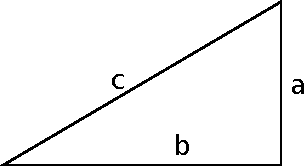
\includegraphics[width=.5\linewidth]{triangle1}
  \caption{A triangle with letters} \label{triangle}
 \end{figure}
 
 


 
 
 \chapter{Experiments}
 
 When trying to draw a rectangled triangle, my program comes up with Figure \ref{triangle2} that is neither rectangled nor a triangle.
 
  \begin{figure}[h]\centering
  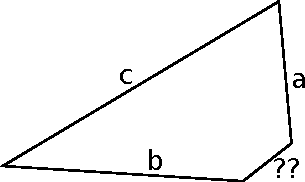
\includegraphics[width=.5\linewidth]{triangle2}
  \caption{Triangle drawn by my program. Note the 4th side.} \label{triangle2}
 \end{figure}
 
Unless there is a bug in my program, which is unlikely, this research indicates that the whole theory on triangles having 3 sides has been wrong for years, maybe decades.
 
 \chapter*{Conclusion}
 \addcontentsline{toc}{chapter}{Conclusion}
 
 
 
 
 
 % switch to A-B-C chaptering
 \appendix	
 
 \chapter{Proof of theorem \ref{theo}}
 \label{sec:prooftheorem}
 
 
 \begin{proof}
\eqref{theo} was already demonstrated in \cite{euclides300}.
\end{proof}
 
 \addcontentsline{toc}{chapter}{Bibliography}
 
 \bibliography{../biblio}
 
 
 
 
\end{document}
